The third iteration is the final development stage of the project. It builds on the observations from the first two iterations and aims to turn the earlier prototypes into a more complete and usable system. The first iteration established that the basic workflow of generating \textit{lilypond} code from \textit{python} was workable, and the second iteration introduced a more meaningful musical object model. The purpose of the third iteration is to bring those lessons together into a generator where form, harmony, range, and rendering belong to the same coherent workflow.

This is also the stage where \ac{AI} is introduced directly into the development process. By waiting until the earlier iterations had already exposed the central musical and technical problems, it became possible to use \ac{AI} support more deliberately. The point was not to let it define the musical direction of the system, but to use it while refining and extending a design that was already understood well enough to evaluate critically.

\section{Development workflow}

  As mentioned earlier, the third iteration is the first stage of the project where \ac{AI} is used directly as part of the implementation work. This was a natural point to introduce it, because the earlier iterations had already revealed the main weaknesses in both the musical output and the software structure. That meant the development could focus less on discovering the problem and more on improving a known design.

  Codex was chosen as the main \ac{AI} tool because it is designed specifically for software engineering work rather than only general chat interaction \cite{CodexAICoding,CodexNowGenerally2026}. In practical terms, this means it is suited to reading an existing code base, proposing or implementing code changes, supporting refactoring, and helping work through design alternatives in context. Those capabilities are especially relevant here, since the main challenge in the final iteration is not simply to generate more code, but to reshape the earlier prototypes into a more structured musical system.

  The role of Codex in this iteration is therefore as a development aid rather than a substitute for musical or architectural judgment. It was useful for acceleration, exploration, and implementation support, while the overall design choices, the musical evaluation of the outputs, and the direction of the system remained under human control. In that sense, the use of \ac{AI} belongs inside the iterative development process rather than standing apart from it.

\section{Software architecture}

  In Figure~\ref{fig:iter3_architecture} we can see how the system is built and how the different modules interact. Compared with the earlier iterations, the third iteration is no longer organized around one large entry script. The command-line workflow has been moved into its own module, while the main entry point is used to define the default configuration of the generator, such as the weighting of the soft constraints. This makes the architecture easier to understand and easier to adapt.

  \begin{figure}[htbp] % Architecture
    \centering
    \begin{adjustbox}{max width=\textwidth,max totalheight=0.85\textheight}
    \begin{tikzpicture}[
      >=Latex,
      font=\normalsize,
      scale=1,
      transform shape,
      node distance=8mm and 10mm,
      stage/.style={
        draw,
        rounded corners=3pt,
        align=center,
        minimum width=0.42\textwidth,
        minimum height=10mm,
        fill=gray!8
      },
      support/.style={
        draw,
        rounded corners=3pt,
        align=center,
        minimum width=0.24\textwidth,
        minimum height=9mm,
        fill=blue!6
      },
      output/.style={
        draw,
        rounded corners=3pt,
        align=center,
        minimum width=0.24\textwidth,
        minimum height=9mm,
        fill=green!8
      },
      arrow/.style={
        -{Latex[length=2.3mm]},
        thick
      }
    ]

      % Main vertical pipeline
      \node[stage] (input) {User input\\key, mode, bars, seed, texture,\\voice profile, harmony, form};
      \node[stage, below=of input] (mainconfig) {\texttt{code/main.py}\\default configuration,\\constraint weights, and entry point};
      \node[stage, below=of mainconfig] (cli) {\texttt{code/app\_cli.py}\\CLI parsing, harmony/form setup,\\and render mode};
      \node[stage, below=of cli] (settings) {\texttt{GenerationSettings}\\with \texttt{Key}, \texttt{Motif}, \texttt{FormPlan},\\\texttt{HarmonyPlan}, and \texttt{VoiceProfile}};
      \node[stage, below=of settings] (generator) {\texttt{MelodyGenerator}\\candidate generation, beat-resolved harmony,\\motif reuse, and weighted selection};
      \node[stage, below=of generator] (melody) {\texttt{Melody} or \texttt{ChoraleScore}\\events, metadata, harmony plan,\\and selected clefs};
      \node[stage, below=of melody] (render) {\texttt{lilypond.py}\\notation export, rerendering,\\and optional PDF/WAV rendering};

      % Side modules
      \node[support, left=18mm of settings] (structure) {\texttt{structure.py}\\core data model,\\HarmonySpan and ChoraleScore};
      \node[support, right=18mm of settings] (theory) {\texttt{theory.py}\\pitch spelling, Roman numerals,\\transposition and chord tones};
      \node[support, left=18mm of generator] (constraints) {\texttt{constraints.py}\\stepwise motion, leaps, cadence,\\climax, rests, motif and form scoring};
      \node[support, right=18mm of generator] (chorale) {\texttt{chorale.py}\\SATB harmonization from\\the generated soprano line};

      % Outputs
      \node[output, below left=10mm and 10mm of render] (lyfile) {\texttt{.ly} source};
      \node[output, below=10mm of render] (pdf) {cropped \texttt{.pdf}};
      \node[output, below right=10mm and 10mm of render] (audio) {\texttt{.midi} and \texttt{.wav}};

      % Pipeline arrows
      \draw[arrow] (input) -- (mainconfig);
      \draw[arrow] (mainconfig) -- (cli);
      \draw[arrow] (cli) -- (settings);
      \draw[arrow] (settings) -- (generator);
      \draw[arrow] (generator) -- (melody);
      \draw[arrow] (melody) -- (render);

      % Support arrows
      \draw[arrow] (structure.east) -- (settings.west);
      \draw[arrow] (theory.west) -- (settings.east);
      \draw[arrow] (constraints.east) -- (generator.west);
      \draw[arrow] (chorale.west) -- (generator.east);

      % Output arrows
      \draw[arrow] (render) -- (lyfile);
      \draw[arrow] (render) -- (pdf);
      \draw[arrow] (render) -- (audio);

    \end{tikzpicture}%
    \end{adjustbox}
    \caption{Architecture of the third iteration melody generator. The reusable CLI layer in \texttt{app\_cli.py} handles parsing and workflow concerns, while \texttt{main.py} defines the default constraint configuration. The generator then combines beat-resolved harmony with a soft-constraint stack, and the resulting melody or chorale is exported through LilyPond into notation and audio assets.}\label{fig:iter3_architecture}
  \end{figure}

  A useful way to think about the third iteration is that the code is now divided into clearer layers of responsibility. The top layer handles configuration and user interaction through \texttt{main.py} and \texttt{app\_cli.py}. Beneath that is a representation layer, where the requested task is gathered into a \texttt{GenerationSettings} object together with explicit musical structures such as keys, harmony plans, form plans, motifs, and voice profiles. Only after that does the actual generation layer begin, and once the result has been produced it passes into a separate export layer through \texttt{lilypond.py}. This is a much more deliberate organization than in the first two iterations, where several of these concerns were mixed together.

  Another important difference from the second iteration is that the architectural boundary between user input and musical generation is more explicit. In the second iteration the script still moved rather directly from a few fixed values to phrase generation. In the third iteration, the separate user choices are first collected and normalized before any pitch generation begins. That may sound like a technical detail, but it is significant, because it means the generator can work from a stable description of the task rather than from scattered assumptions. The same core generator can therefore be reused with different keys, forms, textures, rhythmic vocabularies, and harmonic plans without rewriting the surrounding workflow.



  The figure also shows that the side modules are no longer just utility files, but important parts of the architecture. The data model in \texttt{structure.py} defines the musical objects the rest of the system depends on, while \texttt{theory.py} handles pitch spelling, transposition, Roman numeral interpretation, and chord-tone logic. The constraint layer is also much more central than before. Instead of only restricting a few intervals, \texttt{constraints.py} participates directly in candidate evaluation by scoring melodic motion, harmonic fit, cadence behaviour, climax placement, rest handling, and motivic similarity. This means that the architecture is not only more modular, but also more musical, since the modules correspond more closely to distinct musical tasks.

  It is also worth noting that melody generation and chorale generation now belong to the same overall pipeline. The system first produces a melodic result with its formal and harmonic context intact, and only then, when requested, passes that material into \texttt{chorale.py} for four-part realization. That is a cleaner architecture than treating harmonization as a separate script, because both single-line and multi-voice results depend on the same settings object, the same harmonic description, and the same rendering workflow. In practice this makes the final system feel less like a collection of disconnected experiments and more like one program with a shared musical model.

\section{Implementation}
The most important change in the third iteration is not only that the system got larger, but that the internal representation became detailed enough to support actual musical reasoning. In the first iteration the program mainly handled notes inside a key, and in the second iteration it added motifs, bars, and phrases. In the third iteration, the object model was extended further to include explicit event objects, form sections, harmony spans, and voice profiles. This gives the generator a much clearer description of the musical situation it is working in.

Figure~\ref{fig:iter3_object_model} summarizes this richer object model. Compared with the second iteration, the system now gathers the task into a dedicated settings object and distinguishes more clearly between the structures used during generation and the resulting melody or chorale output.

\begin{figure}[htbp]
  \centering
  \resizebox{\textwidth}{!}{%
  \begin{tikzpicture}[
    >=Latex,
    font=\small,
    node distance=11mm and 12mm,
    class/.style={
      draw,
      rounded corners=3pt,
      align=left,
      fill=gray!8,
      minimum width=38mm
    },
    support/.style={
      draw,
      rounded corners=3pt,
      align=left,
      fill=blue!6,
      minimum width=34mm
    },
    arrow/.style={-{Latex[length=2.3mm]}, thick}
  ]
    \node[class] (settings) {
      \textbf{GenerationSettings}\\
      key\\
      bars\\
      allowed durations\\
      range\\
      form plan\\
      harmony plan\\
      texture\\
      voice profile\\
      chorale plan
    };

    \node[support, left=of settings] (motif) {
      \textbf{Motif}\\
      events: NoteEvent[]
    };

    \node[support, above right=of settings] (form) {
      \textbf{FormPlan}\\
      sections: FormSection[]
    };

    \node[support, right=of settings] (harmony) {
      \textbf{HarmonyPlan}\\
      spans: HarmonySpan[]
    };

    \node[support, right=of harmony] (span) {
      \textbf{HarmonySpan}\\
      start bar / beat\\
      end bar / beat\\
      Roman symbol
    };

    \node[support, above left=of settings] (voice) {
      \textbf{VoiceProfile}\\
      range\\
      tessitura\\
      clef hint
    };

    \node[class, below=24mm of settings] (melody) {
      \textbf{Melody}\\
      events: NoteEvent[]\\
      key\\
      metadata\\
      clef
    };

    \node[class, right=of melody] (chorale_result) {
      \textbf{ChoraleScore}\\
      soprano\\
      alto\\
      tenor\\
      bass\\
      harmony plan
    };

    \node[support, left=of melody] (event) {
      \textbf{NoteEvent}\\
      scale step\\
      duration\\
      chromatic adjustment\\
      rest flag
    };

    \draw[arrow] (motif) -- (settings);
    \draw[arrow] (form) -- (settings);
    \draw[arrow] (harmony) -- (settings);
    \draw[arrow] (span) -- (harmony);
    \draw[arrow] (voice) -- (settings);
    \draw[arrow] (settings) -- node[left] {used in generating} (melody);
    \draw[arrow] (settings) -- node[right] {also drives} (chorale_result);
    \draw[arrow] (event) -- node[above] {used in} (melody);
    \draw[arrow] (motif) -- node[left] {reused as} (event);
  \end{tikzpicture}%
  }
  \caption{Simplified object model of the third iteration. Compared with the earlier iterations, musical information is no longer limited to notes and phrases, but also includes beat-resolved harmony spans, texture settings, voice profiles, rests, and a separate chorale result type.}
  \label{fig:iter3_object_model}
\end{figure}


The short code excerpt below shows an important part of that change. Instead of only storing notes and durations, the third iteration introduces objects that describe vocal range, formal function, and motivic material directly in the data model.

\lstinputlisting[language=Python]{code/iter3_structure_excerpt.py}

This is a more useful view of the third iteration than a very small note object on its own. \texttt{VoiceProfile} gives the generator a way to talk about range and tessitura, \texttt{FormSection} describes the role of each part of the phrase, and \texttt{Motif} makes it possible to store a musical cell as an object instead of only reproducing it procedurally. Taken together, these structures show that the third iteration is not just generating more notes, but reasoning about richer musical objects.

Another important improvement is that the generation task is gathered into a single settings object. Rather than relying on hard-coded assumptions spread across one large script, the third iteration collects key, form, harmony, durations, range, and voice information before generation starts, while leaving the default weighting of the musical constraints in the main entry point. This makes the system easier to extend and also makes the constraints easier to apply consistently.

It is also useful to follow what the system actually does after a command is received. The first step is shown in Figure~\ref{fig:iter3_setup_flow}. The command line is parsed in \texttt{app\_cli.py}, and the separate user choices are then collected into a single \texttt{GenerationSettings} object. This is where the key, time signature, form plan, harmony plan, motif, texture, and voice profile are brought together into one consistent description of the task.

\begin{figure}[htbp]
  \centering
  \resizebox{0.92\textwidth}{!}{%
  \begin{tikzpicture}[
    >=Latex,
    font=\small,
    node distance=10mm and 8mm,
    stage/.style={
      draw,
      rounded corners=3pt,
      align=center,
      minimum width=0.25\textwidth,
      minimum height=9mm,
      fill=gray!8
    },
    arrow/.style={-{Latex[length=2.2mm]}, thick}
  ]
    \node[stage] (cmd) {CLI command\\key, bars, form, harmony, seed, texture};
    \node[stage, right=of cmd] (cli) {\texttt{app\_cli.py}\\parse arguments and validate input};
    \node[stage, right=of cli] (settings) {\texttt{GenerationSettings}\\key, motif, form plan,\\harmony plan, and voice profile};

    \draw[arrow] (cmd) -- (cli);
    \draw[arrow] (cli) -- (settings);
  \end{tikzpicture}%
  }
  \caption{The first stage of the third iteration. The command line is parsed and translated into a single structured settings object before any music is generated.}
  \label{fig:iter3_setup_flow}
\end{figure}


Once the settings are ready, the melody generator begins to prepare the musical context before it commits to any pitches. Figure~\ref{fig:iter3_melody_flow} shows this middle stage. The generator first creates a rhythmic skeleton that fits the number of bars and the phrase layout. It then decides where the motif should return and where the melodic climax should be placed. Only after those larger targets are set does it begin to choose notes.

\begin{figure}[htbp]
  \centering
  \resizebox{0.95\textwidth}{!}{%
  \begin{tikzpicture}[
    >=Latex,
    font=\small,
    node distance=9mm and 8mm,
    stage/.style={
      draw,
      rounded corners=3pt,
      align=center,
      minimum width=0.22\textwidth,
      minimum height=9mm,
      fill=gray!8
    },
    arrow/.style={-{Latex[length=2.2mm]}, thick}
  ]
    \node[stage] (rhythm) {Build rhythm\\bar durations and phrase endings};
    \node[stage, right=of rhythm] (targets) {Choose targets\\motif returns and climax position};
    \node[stage, right=of targets] (candidates) {For each event\\find harmony and make candidates};
    \node[stage, right=of candidates] (score) {Score attempts\\soft constraints and best attempt};

    \draw[arrow] (rhythm) -- (targets);
    \draw[arrow] (targets) -- (candidates);
    \draw[arrow] (candidates) -- (score);
  \end{tikzpicture}%
  }
  \caption{The melody-generation stage in the third iteration. The generator first decides structural targets, then evaluates candidate notes under the active harmonic and formal context.}
  \label{fig:iter3_melody_flow}
\end{figure}


Figure~\ref{fig:iter3_process_rhythm} illustrates this idea using the opening of one real third-iteration output. At this stage the interesting information is not yet the pitch contour, but the rhythmic shape and the bar structure. The generator has already committed to note lengths and phrase pacing, which means the later pitch decisions will happen inside a more stable framework.

\begin{figure}[htbp]
  \centering
  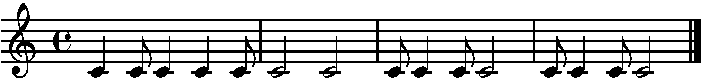
\includegraphics[width=0.85\textwidth]{examples/iter3/iter3_process_rhythm.cropped.pdf}
  \caption{A rhythmic skeleton corresponding to the first four bars of a generated third-iteration melody. At this stage the durations and bar structure are fixed, while the actual pitch content is still to be chosen.}
  \label{fig:iter3_process_rhythm}
\end{figure}

The pitch generation itself happens as a repeated local decision process. For each event position, the code looks up the current bar, beat, harmony span, and form role, and then builds a group of candidate notes around the existing melodic context. These candidates are scored by the soft-constraint stack, which considers things such as stepwise motion, leap recovery, harmonic fit, motif similarity, cadence behaviour, and the general melodic shape. Rather than simply walking around the scale, the third iteration repeatedly asks what would make musical sense at this exact point in the phrase.

The next code excerpt shows that process more directly. Rather than showing the whole function, it shows the essential step: a context object is assembled for the current note, and the candidate is chosen against that context.

\lstinputlisting[language=Python, breaklines=true, breakatwhitespace=true]{code/iter3_generation_excerpt.py}

The result of that process is shown in Figure~\ref{fig:iter3_process_melody}. Here the same rhythmic outline has been given actual pitches, and the opening four bars now begin to show the musical character of the line. This makes the implementation easier to follow because it shows how the final melody is not generated all at once, but emerges from rhythm, context, and repeated local choices.

\begin{figure}[htbp]
  \centering
  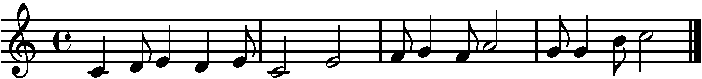
\includegraphics[width=0.85\textwidth]{examples/iter3/iter3_process_melody.cropped.pdf}
  \caption{The same opening after pitch generation. The rhythmic framework has now been turned into a concrete melody by repeated candidate evaluation under the active harmonic and formal context.}
  \label{fig:iter3_process_melody}
\end{figure}

The final melody is selected from several complete attempts rather than from one single pass. After that, the workflow splits as shown in Figure~\ref{fig:iter3_output_flow}. If the requested texture is just a melody, the resulting line is exported directly. If the texture is chorale, the melody is treated as a soprano line and passed to the harmonizer, which chooses alto, tenor, and bass notes according to the same harmony plan and the SATB voice profiles. The last step in both cases is export through LilyPond, with optional PDF, MIDI, and WAV rendering.

\begin{figure}[htbp]
  \centering
  \resizebox{0.92\textwidth}{!}{%
  \begin{tikzpicture}[
    >=Latex,
    font=\small,
    node distance=10mm and 12mm,
    stage/.style={
      draw,
      rounded corners=3pt,
      align=center,
      minimum width=0.23\textwidth,
      minimum height=9mm,
      fill=gray!8
    },
    output/.style={
      draw,
      rounded corners=3pt,
      align=center,
      minimum width=0.2\textwidth,
      minimum height=9mm,
      fill=green!8
    },
    arrow/.style={-{Latex[length=2.2mm]}, thick}
  ]
    \node[stage] (melody) {Best melody};
    \node[output, right=of melody] (single) {\texttt{Melody}\\export directly};
    \node[stage, below=of melody] (chorale) {\texttt{ChoraleHarmonizer}\\choose alto, tenor, bass};
    \node[output, right=of chorale] (satb) {\texttt{ChoraleScore}\\SATB export};
    \node[stage, right=28mm of single] (render) {\texttt{lilypond.py}\\PDF, MIDI, WAV};

    \draw[arrow] (melody) -- (single);
    \draw[arrow] (melody) -- (chorale);
    \draw[arrow] (chorale) -- (satb);
    \draw[arrow] (single) -- (render);
    \draw[arrow] (satb) -- (render);
  \end{tikzpicture}%
  }
  \caption{The final stage of the workflow. The best melody can either be exported directly or used as soprano input for chorale harmonization before rendering.}
  \label{fig:iter3_output_flow}
\end{figure}


Figure~\ref{fig:iter3_process_chorale} shows the final branch where the melody is no longer kept as a single line, but is instead used as the soprano basis for a simple SATB-style texture. This figure is especially useful because it shows that the third iteration does not only improve the quality of isolated melodies, but also provides enough harmonic and structural information to support a later harmonization stage.

\begin{figure}[htbp]
  \centering
  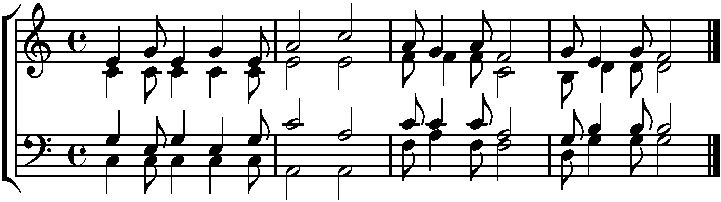
\includegraphics[width=0.9\textwidth]{examples/iter3/iter3_process_chorale.cropped.pdf}
  \caption{The same musical material after chorale harmonization. The generated melody is treated as a soprano line, and alto, tenor, and bass voices are chosen against the same harmonic plan.}
  \label{fig:iter3_process_chorale}
\end{figure}

\section{Results}
The musical output of the third iteration is noticeably more controlled than in the previous versions. The melodies remain within a defined vocal or instrumental range, the generator can take a harmonic plan into account, and motif reuse is no longer limited to literal repetition. The addition of form planning also makes it possible to think in larger units such as sentences and periods rather than only local note-to-note movement.

The examples below show different capabilities of the software. One example for a basic melody result, one for explicit form handling, one for rhythmic restriction, one for alternative choral scoring, and one final longer example showing what can be done when the user gives the system a more detailed harmonic plan.

The first capability is simply that the generator now produces a usable single-line melody. Example~\ref{fig:iter3_melody_1} shows an ordinary output in C major using the default settings. Compared with the first two iterations, the important point is not that the melody is perfect, but that it remains within range, reuses material in a more deliberate way, and arrives at a cadence that feels shaped rather than accidental.

\begin{example}
  \begin{center}
    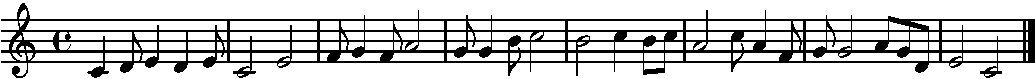
\includegraphics[width=0.95\textwidth]{examples/iter3/iter3_melody_1.cropped.pdf}
  \end{center}
  \caption[A melody generated by the third iteration in C major.]{A melody generated by the third iteration in C major, showing a sentence-like shape with clear motivic reuse. \examplelink.}\label{fig:iter3_melody_1}
\end{example}

The second capability is explicit form control. This becomes easier to observe when the melody is allowed to unfold over a larger span. Example~\ref{fig:iter3_period_16_d} shows a 16-bar melody in D major generated using the \texttt{period} form plan. In this case the balanced phrase structure and the different treatment of the return toward cadence are easier to recognize than in the shorter examples, and this makes it clearer that the generator is no longer only producing note-to-note movement, but is instead working with a larger formal outline.

\begin{example}
  \begin{center}
    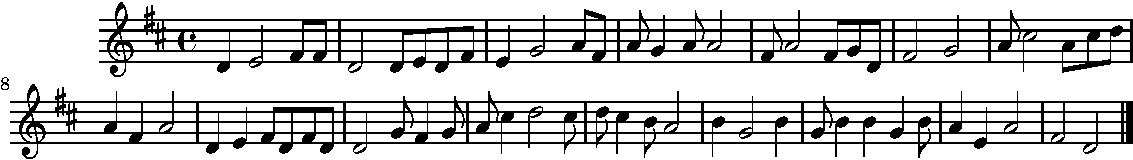
\includegraphics[width=0.95\textwidth]{examples/iter3/iter3_period_16_d.cropped.pdf}
  \end{center}
  \caption[A 16-bar period-form melody generated by the third iteration in D major.]{A 16-bar melody generated by the third iteration in D major using the explicit \texttt{period} form plan. \examplelink.}\label{fig:iter3_period_16_d}
\end{example}

The third capability is rhythmic restriction. The generator can be given a narrower rhythmic vocabulary, which changes the surface character without changing the larger harmonic and formal workflow. Example~\ref{fig:iter3_rhythm_mixed_a} shows a melody in A major generated using only whole, half, and quarter notes. This is useful because it demonstrates that the rhythmic content can be shaped deliberately instead of always relying on the default mixture of durations.

\begin{example}
  \begin{center}
    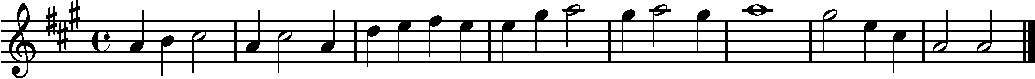
\includegraphics[width=0.95\textwidth]{examples/iter3/iter3_rhythm_mixed_a.cropped.pdf}
  \end{center}
  \caption[A melody in A major generated with restricted rhythm values.]{A melody in A major generated using only whole, half, and quarter notes. \examplelink.}\label{fig:iter3_rhythm_mixed_a}
\end{example}

The fourth capability is flexible scoring. The same harmonization workflow does not have to be limited to a standard SATB arrangement. Example~\ref{fig:iter3_chorale_ttbb_g_minor} shows a four-part result in G minor using a TTBB layout. This demonstrates that the harmonization layer can be adapted to other ensemble requirements, as long as appropriate voice profiles are provided.

\begin{example}
  \begin{center}
    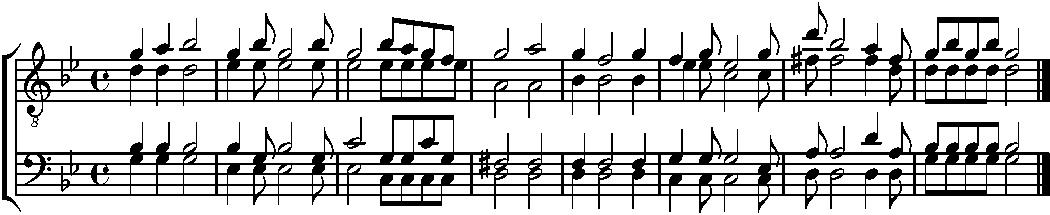
\includegraphics[width=0.95\textwidth]{examples/iter3/iter3_chorale_ttbb_g_minor.cropped.pdf}
  \end{center}
  \caption[A TTBB-style harmonized example generated by the third iteration in G minor.]{A four-part TTBB-style example generated by the third iteration in G minor. \examplelink.}\label{fig:iter3_chorale_ttbb_g_minor}
\end{example}

The final capability is explicit harmonic control. This is perhaps the clearest example of how the program can be used differently by someone with more musical knowledge. Instead of relying on the automatic tonal plan, the user can specify a progression directly and use the compact harmony syntax to shape the result bar by bar and beat by beat. Example~\ref{fig:iter3_long_explicit_chorale_bb} shows a longer 16-bar chorale in B$\flat$ major using an explicit progression with borrowed chords such as \texttt{iv} and \texttt{bVII}. This kind of input allows the output to move beyond the most standard diatonic patterns and makes the system feel more like a compositional tool than only a generator of default examples.

\begin{example}
  \begin{center}
    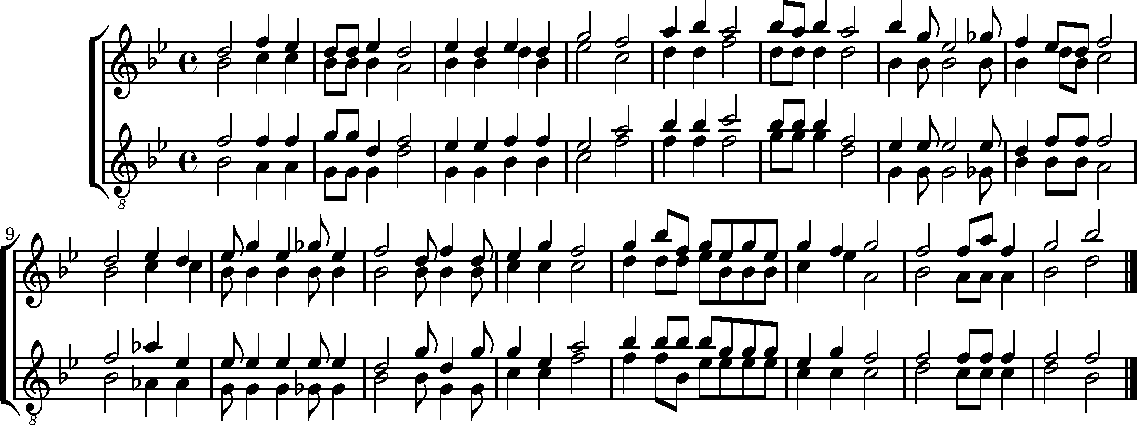
\includegraphics[width=0.95\textwidth]{examples/iter3/iter3_long_explicit_chorale_bb.cropped.pdf}
  \end{center}
  \caption[A 16-bar explicit-harmony chorale generated by the third iteration in B$\flat$ major with modal mixture.]{A 16-bar harmonized example generated by the third iteration in B$\flat$ major using an explicit harmonic progression with the borrowed \texttt{iv} and \texttt{bVII} chords. This is the kind of output that becomes possible when the user approaches the program with a more deliberate harmonic idea. \examplelink.}\label{fig:iter3_long_explicit_chorale_bb}
\end{example}

Another clear improvement is that the notation workflow became much more usable. The system can now place generated files in seed-based output folders, choose a clef more intelligently, and optionally render cropped PDF files and audio from the same command-line call. This does not change the melody itself, but it makes the generator much easier to use as part of a real compositional and thesis-writing workflow.

Even with these improvements, the results are still heuristic rather than guaranteed. The generator is better at preferring musically convincing solutions, but it does not prove that every melody will be good. The value of the third iteration is therefore that it makes good results much more likely while also making the failures easier to understand and improve. The appendix can be read as an extended version of this results section, where the same capabilities are shown across more keys, more rhythm settings, and more texture choices.

\section{Discussion}
The third iteration is the first version where the musical objects and the generation strategy point in the same direction. In the earlier iterations the generator could produce output, but the internal representation was too weak to carry much musical meaning. Here, the object model is rich enough that concepts such as form, harmony, range, and motif transformation can be represented directly in the code instead of only being implied by the generation procedure.

The most important improvement is therefore not only that the output is better, but that the reasons for the output are easier to understand. A melody can now be discussed in terms of its form plan, harmonic context, rhythmic vocabulary, and voice profile, because those things exist explicitly in the system. This makes the successes more meaningful, but it also makes the failures easier to diagnose. If a phrase feels weak, it is now possible to ask whether the problem lies in the form handling, the candidate scoring, the harmonic plan, or the chosen range, rather than only hearing that the result sounds wrong.

This is also the first iteration that feels like a reusable foundation rather than only an experiment. Because the settings, structure, theory, and constraint layers are separated more clearly, the system can be extended without rewriting the entire program. That is especially important for later work such as more robust four-part writing, since multi-voice generation requires a representation that can handle range, harmonic function, and voice-leading information at the same time.

At the same time, the third iteration still depends heavily on heuristic balancing. The constraint weights are chosen by judgment and testing rather than derived from a formal model, and the quality of the result still depends on how well those weights interact. A setting that works well for one kind of melody may work as well for another, especially when the key, rhythm, or texture changes. The generator is therefore much more controlled than before, but it is not guaranteed to produce a strong result every time.

Another remaining limitation is that the system still makes many of its decisions locally, even though the local choices are informed by a richer context. The generator knows much more about the phrase than in the earlier iterations, but it still does not plan an entire melody in the way a human composer might. Because of this, some results can still contain moments that are individually acceptable but not fully convincing when heard as part of the larger line. The use of several complete attempts helps mitigate this, but it does not remove the problem entirely.

The chorale output should also be understood in that light. It demonstrates that the third iteration has enough harmonic and structural information to support four-part realization, which is a major improvement over the earlier versions. However, the harmonization is still relatively simple compared with a fully developed model of chorale writing. It is useful as a proof that the architecture can support this kind of extension, but there is still room for more detailed control of spacing, doubling, and voice-leading.

Even with these limitations, the third iteration represents a substantial step forward. Compared with the first two iterations, the final version is much closer to a tool that can be discussed, refined, and extended in a systematic way rather than only adjusted by trial and error.
